\documentclass[compress]{beamer}

\mode<presentation>
\usetheme{Madrid}
\definecolor{Columbia}{RGB}{185,217,235}
\definecolor{Columbia2}{RGB}{0,51,160}
\definecolor{Columbia3}{RGB}{0,114,206}
\setbeamercolor{title}{fg=Columbia2}
\setbeamercolor{frametitle}{fg=Columbia2}
\setbeamercolor{block title}{bg=Columbia, fg=Columbia2}
%\setbeamercolor{block body}{fg=Columbia2}
\setbeamercolor{structure}{fg=Columbia}
\setbeamercolor{item projected}{fg=white}
\setbeamercolor{item}{fg=Columbia2}
\setbeamercolor{subitem}{fg=Columbia2}
\setbeamercolor{section in toc}{fg=Columbia2}
\setbeamercolor{description item}{fg=Columbia}
\setbeamercolor{caption name}{fg=Columbia2}
\setbeamercolor{button}{fg=Columbia2}
\usepackage{graphics}
\usepackage{geometry}
\usepackage{booktabs}
\usepackage{tikz}
\usepackage{amsmath}
\usepackage{bbm}
\usetikzlibrary{decorations.pathreplacing}
\usepackage{multirow, makecell}
\usepackage{float}
\usepackage{fancyvrb}
\usepackage{caption}
\usepackage{subcaption}
\usepackage{adjustbox}
\usepackage{threeparttable}
\usepackage{hyperref}
\usepackage[scaled=0.92]{helvet}
\newenvironment{wideitemize}{\itemize\addtolength{\itemsep}{10pt}}{\enditemize}
\newenvironment{wideenumerate}{\enumerate\addtolength{\itemsep}{10pt}}{\endenumerate}
%\hypersetup{
%colorlinks=true,
%linkcolor=black,
%filecolor=green, 
%urlcolor=blue,
%}
\beamertemplatenavigationsymbolsempty
\setbeamercolor{author in head/foot}{bg=Columbia2, fg=white}
\setbeamercolor{title in head/foot}{bg=Columbia3, fg=white}
\setbeamercolor{date in head/foot}{bg=Columbia, fg=Columbia2}
\setbeamercolor{section in head/foot}{bg=Columbia, fg=Columbia2}
\setbeamercolor{headline}{bg=Columbia}
\setbeamertemplate{footline}{
    \leavevmode%
    \hbox{%
        \begin{beamercolorbox}[wd=.333333\paperwidth,ht=2.25ex,dp=1ex,center]{author in head/foot}%
            \usebeamerfont{author in head/foot}\insertshortauthor
        \end{beamercolorbox}%
        \begin{beamercolorbox}[wd=.333333\paperwidth,ht=2.25ex,dp=1ex,center]{title in head/foot}%
            \usebeamerfont{title in head/foot}\insertshorttitle
        \end{beamercolorbox}%
        \begin{beamercolorbox}[wd=.333333\paperwidth,ht=2.25ex,dp=1ex,right]{date in head/foot}%
            \usebeamerfont{date in head/foot}\insertshortdate{}\hspace*{2em}
            \insertframenumber{} / \inserttotalframenumber\hspace*{2ex} 
        \end{beamercolorbox}}%
        \vskip0pt%
    }
\setbeamercolor{page number in head/foot}{fg=black}
\setbeamertemplate{section in toc}[sections numbered]
\setbeamertemplate{subsection in toc}{\leavevmode\leftskip=3em\rlap{\hskip-1.75em\inserttocsectionnumber.\inserttocsubsectionnumber}\inserttocsubsection\par}
\setbeamerfont{subsection in toc}{size=\footnotesize}
%\setbeamertemplate{headline}{%
  %\begin{beamercolorbox}[ht=5.5ex]{section in head/foot}
    %\vskip2pt\insertnavigation{0.33\paperwidth}\vskip2pt
  %\end{beamercolorbox}%
%}


\makeatletter
\let\@@magyar@captionfix\relax
\makeatother


\title[Recitation 4]{Recitation 4} % Change this regularly
\author[Seung-hun Lee]{Seung-hun Lee}
\institute[Columbia University]{Columbia University}

\date[]{}

\begin{document}
\begin{frame}
\titlepage
\end{frame}

%%%%%%%%%%%%% Section 1. 


% Capture in one slide
% Separate slide for questions
\begin{frame}
\frametitle{Ordinary Least Squares}
Sampling distribution 
\begin{itemize}
\item OLS estimate that we are getting is a random variable - getting different estimates depending on sample we work with. 
\item$\hat{\beta}_1$: Recall that we can write
\[
\hat{\beta}_1= \frac{\sum_{i=1}^n(X_i-\bar{X})(Y_i-\bar{Y})}{\sum_{i=1}^n(X_i-\bar{X})^2}
\]
Now, replace $Y_i$ an $\bar{Y}$ with 
\[
Y_i =\beta_0 + \beta X_i + u_i, \ \bar{Y} = \beta_0 + \beta_1\bar{X} + \bar{u},
\]
which allows us to write 
\[
(Y_i-\bar{Y}) = (\beta_1(X_i-\bar{X})+(u_i-\bar{u}))
\]
and get
\[
\hat{\beta}_1=\beta_1+  \frac{\sum_{i=1}^n(X_i-\bar{X})(u_i-\bar{u})}{\sum_{i=1}^n(X_i-\bar{X})^2}
\]

\end{itemize}
\end{frame}

\begin{frame}
\frametitle{Ordinary Least Squares}
\begin{itemize}
\item $E[\hat{\beta}_1]$: It can be written as
\small{\[
\begin{aligned}
E[\hat{\beta}_1]& = E\left[\beta_1+  \frac{\sum_{i=1}^n(X_i-\bar{X})(u_i-\bar{u})}{\sum_{i=1}^n(X_i-\bar{X})^2}\right]\\
&=\beta_1+ E\left[\frac{\sum_{i=1}^n(X_i-\bar{X})(u_i-\bar{u})}{\sum_{i=1}^n(X_i-\bar{X})^2}\right]
\end{aligned}
\]}\normalsize
$\sum_{i=1}^n(X_i-\bar{X})(u_i-\bar{u})$ can be written to something simpler.
\small{\[
\sum_{i=1}^n(X_i-\bar{X})(u_i-\bar{u})=\sum_{i=1}^nX_iu_i-\bar{u}\sum_{i=1}^n X_i+\bar{X}\sum_{i=1}^nu_i+n\bar{X}\bar{u}
\]}\normalsize
\item[$\to$] Since $\bar{X}$ is a sample mean of $X$, $\sum_{i=1}^nX_i=n\bar{X}$. \\
\item[$\to$] The assumption that conditional mean is zero and $(X_i, u_i)$ are uncorrelated means that the term on the left hand side is zero. 
\item[$\to$] Therefore, UNDER CLASSICAL ASSUMPTIONS, $E[\hat{\beta}_1]=\beta_1$.

\end{itemize}
\end{frame}

\begin{frame}
\frametitle{Ordinary Least Squares}
\begin{itemize}
\item $var[\hat{\beta}_1]$: We use the definition of the variances and the fact that the expected value of $\hat{\beta}_1$ is unbiased (at least for now) to get
\[
\begin{aligned}
var(\hat{\beta}_1)&=E\left[\left(\hat{\beta}_1-E[\hat{\beta}_1]\right)^2\right] \\
&=E\left[\left(\hat{\beta}_1-{\beta}_1\right)^2\right]\\
&=E\left[\left( \frac{\sum_{i=1}^n(X_i-\bar{X})(u_i-\bar{u})}{\sum_{i=1}^n(X_i-\bar{X})^2} \right)^2\right]\\
&=E\left[\left(  \frac{(X_1-\bar{X})(u_1-\bar{u})}{\sum_{i=1}^n(X_i-\bar{X})^2}+...+\frac{(X_n-\bar{X})(u_n-\bar{u})}{\sum_{i=1}^n(X_i-\bar{X})^2} \right)^2\right]\\
\end{aligned}
\]
\end{itemize}
\end{frame}

\begin{frame}
\frametitle{Ordinary Least Squares}
\begin{itemize}
\item[$\to$] We assume homoskedasticity and no autocorrelation
\item[$\to$] Since $X_i$ is from the data and $u_i$ is a random error term, we can take all the $X_i$ terms in and keep the $u_i$ terms in the expectation to get (i.i.d assumption is also useful here)
\[
\begin{aligned}
var(\hat{\beta}_1)&=\frac{\sum_{i=1}^n(X_i-\bar{X})^2E[(u_i-\bar{u})^2]}{[\sum_{i=1}^n(X_i-\bar{X})^2]^2}\\
&=\frac{\sum_{i=1}^n(X_i-\bar{X})^2\sigma_u^2}{[\sum_{i=1}^n(X_i-\bar{X})^2]^2} \ (\because E[(u_i-\bar{u})^2=var(u_i))\\
&=\sigma_u^2\frac{\sum_{i=1}^n(X_i-\bar{X})^2}{[\sum_{i=1}^n(X_i-\bar{X})^2]^2} =\frac{\sigma_u^2}{\sum_{i=1}^n(X_i-\bar{X})^2}
\end{aligned}
\]
Note that  to decrease the variance in the estimates, the variance of the error should be small relative to the variation in the $X_i$. 
\end{itemize}
\end{frame}

\begin{frame}
\frametitle{Ordinary Least Squares}
\begin{itemize}
\item $\hat{\beta}_0$: The formula for $\hat{\beta}_0$ is $\bar{Y}-\hat{\beta}_1\bar{X}$. By changing $\bar{Y}$, we can get
\[
\begin{aligned}
\hat{\beta}_0&=(\beta_0+\beta_1\bar{X}+\bar{u})-\hat{\beta}_1\bar{X}\\
&=\beta_0+(\beta_1-\hat{\beta}_1)\bar{X}+\bar{u}
\end{aligned}
\]
Then we can say the following about the sampling distribution
\item $E[\hat{\beta}_0]$: We can write
\[
E[\hat{\beta}_0]=\beta_0+E[(\beta_1-\hat{\beta}_1)\bar{X}]+E[\bar{u}]=\beta_0
\]
since $\hat{\beta}_1$ is unbiased and conditional expectation of $u_i$ is zero. 
\item[$\to$]Thus, under our current assumptions, $\hat{\beta}_0$ is unbiased. 
\end{itemize}
\end{frame}

\begin{frame}
\frametitle{Ordinary Least Squares}
\begin{itemize}
\item $var[\hat{\beta}_0]$: Using the definition of the variance, we can write \[
\begin{aligned}
var(\hat{\beta}_0)&=E\left[\left(\hat{\beta}_0-E[\hat{\beta}_0]\right)^2\right] =E\left[\left(\hat{\beta}_0-{\beta}_0\right)^2\right]\\
&=E\left[\left( (\beta_1-\hat{\beta}_1)\bar{X}+\bar{u}\right)^2\right]\\
&=\bar{X}^2E\left[\left(\beta_1-\hat{\beta}_1 \right)^2\right]+ 2\bar{X}E\left[\left(\beta_1-\hat{\beta}_1 \right)\bar{u}\right] + E[\bar{u}^2]
\end{aligned}
\]
Under the assumption (A2), we can ignore the middle term as this is zero. The rest of the terms are $\bar{X}^2 var(\hat{\beta}_1)$ and $\frac{\sigma_u^2}{n}$. the final result is
\[
var(\hat{\beta}_0)=\frac{\sigma_u^2\bar{X}^2}{\sum_{i=1}^n(X_i-\bar{X})^2}+\frac{\sigma_u^2}{n}= \frac{\sigma_u^2}{n}\frac{\sum_{i=1}^nX_i^2}{\sum_{i=1}^n(X_i-\bar{X})^2}
\]
\end{itemize}
\end{frame}

\begin{frame}
\frametitle{Ordinary Least Squares}
So what do we take away?
\begin{itemize}
\item At the end of the day, we can say
\begin{gather*}
 \hat{\beta}_1 \sim N\left(\beta_1, \frac{\sigma_u^2}{\sum_{i=1}^n(X_i-\bar{X})^2}\right) \\
\hat{\beta}_0 \sim N\left(\beta_0, \frac{\sigma_u^2}{n}\frac{\sum_{i=1}^nX_i^2}{\sum_{i=1}^n(X_i-\bar{X})^2}\right)
\end{gather*}
\item The importance of this is that now we can conduct a hypothesis test and create a test statistic based on this distribution
\end{itemize}
\end{frame}

\begin{frame}
\frametitle{Ordinary Least Squares}
Hypothesis test
\begin{itemize}
\item From the sample distribution of $\hat{\beta}_1$, we can break down into two cases
\item \textbf{Know $\sigma_u$}: Since the $\hat{\beta}_1$ takes a normal distribution, we can ``standardize" it to get the test statistic and the distribution for it
\[
\frac{\hat{\beta}_1-\beta_1}{\sqrt{var(\hat{\beta}_1)}}\sim N(0,1)
\]
and compare against the critical values (depending on significance level, two vs one-sided test)
\end{itemize}
\end{frame}

\begin{frame}
\frametitle{Ordinary Least Squares}
Hypothesis test
\begin{itemize}
\item \textbf{Don't know $\sigma_u$}; need to have an estimate for $var(\hat{\beta}_1)$ due to not knowing $\sigma_u$. The test statistics and its distribution is
\[
\frac{\hat{\beta}_1-\beta_1}{\sqrt{\widehat{var(\hat{\beta}_1)}}}\sim t_{n-2}
\]
where $\widehat{var(\hat{\beta}_1)}$ is the estimate for the variance and $t_{n-2}$ is a t-distribution with $n-2$ degrees of freedom.
\item The d.f. is determined by the number of observations, where 2 is subtracted because we are estimating $\beta_0$ and $\beta_1$ in the process.
\item When $n$ is large, t-distribution becomes similar to the normal distribution
\end{itemize}
\end{frame}

\begin{frame}
\frametitle{Ordinary Least Squares}
Confidence interval
\begin{itemize}
\item  \textbf{Confidence interval}: A 95\% confidence interval is a range of numbers that form a random interval that has a 95\% chance of including a (nonrandom) true value of a parameter. 
\item This can be obtained by inverting the rejection region that we have used in the critical value approach.
\footnotesize{\begin{gather*}
\Pr\left(-1.96\leq \frac{\hat{\beta}_1-\beta_1}{\sqrt{var(\hat{\beta}_1)}} \leq1.96\right)=0.95\\
\implies \Pr\left(\hat{\beta}_1-1.96\times\sqrt{var(\hat{\beta}_1)} \leq \beta_1 \leq\hat{\beta}_1+1.96\times\sqrt{var(\hat{\beta}_1)}\right)=0.95
\end{gather*}}\normalsize
\item  If they encompass the null test value, then we cannot reject the null hypothesis. Otherwise, we can reject the null. 
\end{itemize}
\end{frame}

\begin{frame}
\frametitle{Ordinary Least Squares}
Binary $X_i$
\begin{itemize}
\item We may be interested in whether there is a difference in outcome due to affiliation to a certain group, which is usually binary
\item \textbf{Dummy variable}: 
\[
X_i = \begin{cases} 1 & \text{if $i$ belongs in group $X$} \\  0 & \text{if otherwise} \\ \end{cases}
\]
\item OLS method can be applied, with different interpretation
\[
\begin{aligned}
E[Y_i |X_i=0]=& \beta_0\\
E[Y_i |X_i=1]=& \beta_1+\beta_0\\
\end{aligned}
\]
$\beta_1$ is then the difference in mean between $X_i=1$ and $X_i=0$ groups
\end{itemize}
\end{frame}

\begin{frame}
\frametitle{Ordinary Least Squares}
Heteroskedasticity
\begin{itemize}
\item The assumption that $var(u_i)$ is constant may not hold.
\item If we stick to homoskedasticity in this case, the standard errors are incorrectly estimated (usually underestimated)
\begin{figure}[H]
\centering
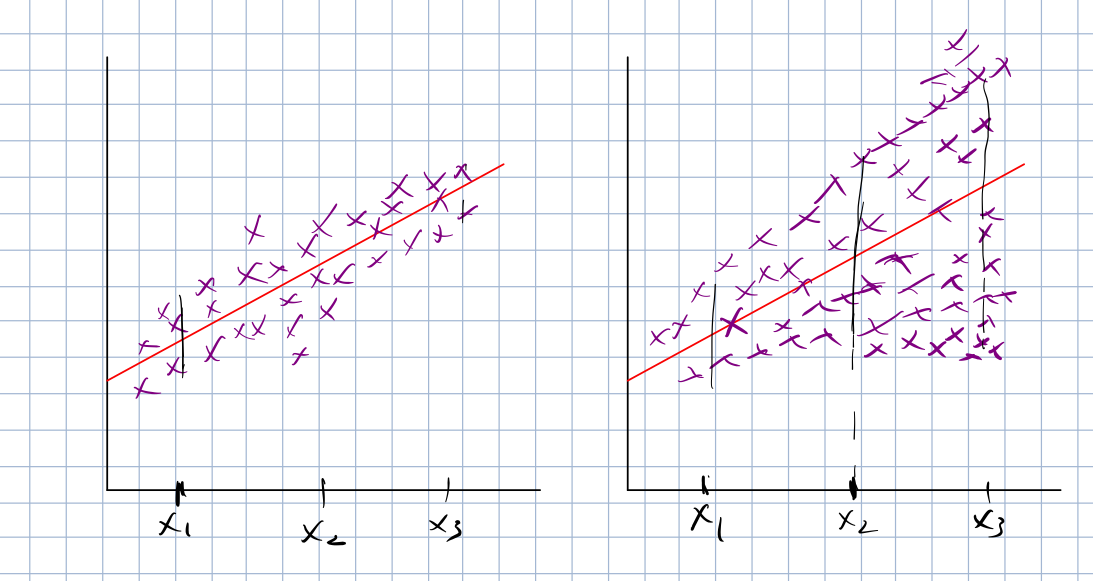
\includegraphics[width=0.55\textwidth]{hetero.png}
\end{figure}
\item  In such case, standard errors of our estimators must take this into account.
\end{itemize}
\end{frame}

\begin{frame}
\frametitle{Ordinary Least Squares}
Consequences of heteroskedasticity
\begin{figure}[H]
\centering
\begin{subfigure}[b]{0.49\textwidth}
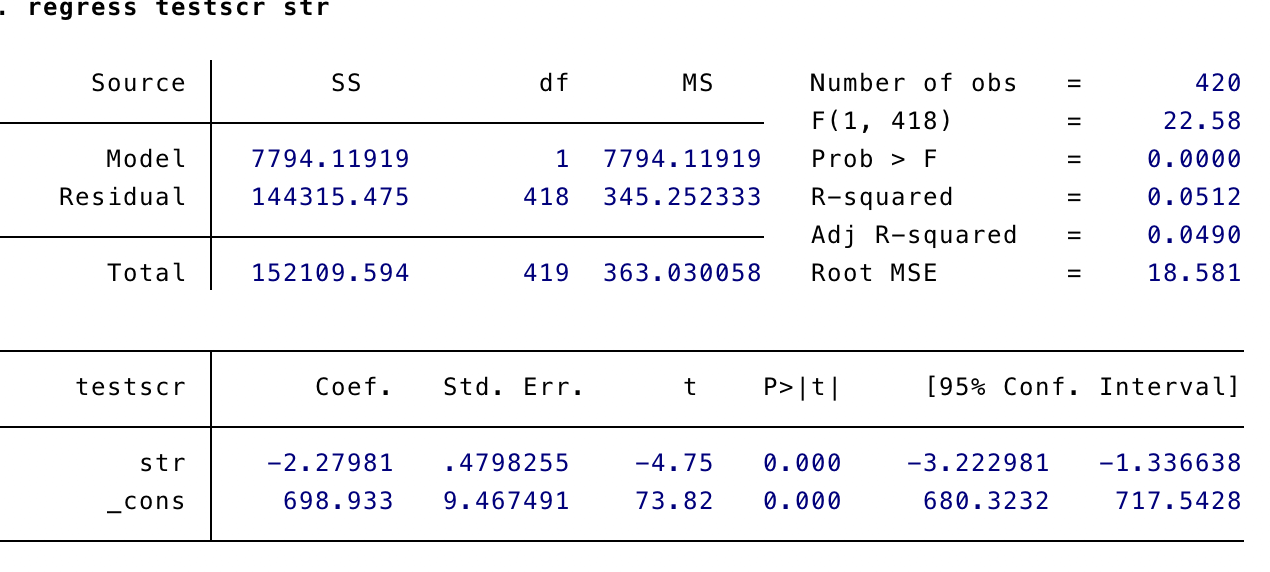
\includegraphics[width=\textwidth]{nonrobust.png}
\end{subfigure}
\begin{subfigure}[b]{0.49\textwidth}
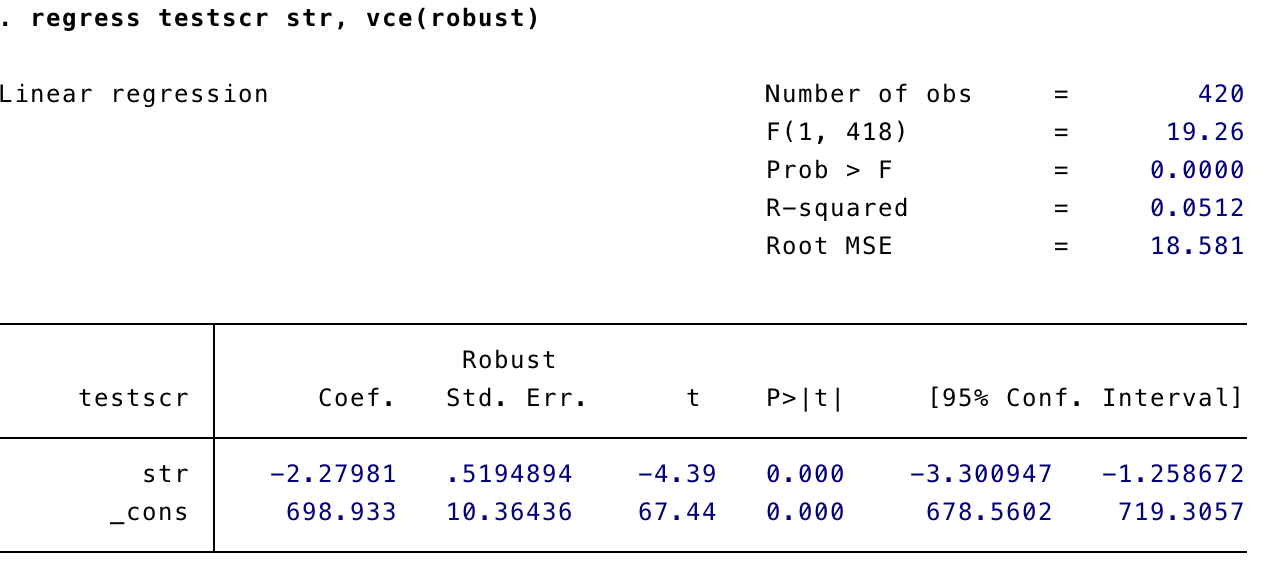
\includegraphics[width=\textwidth]{robust.png}
\end{subfigure}
\end{figure}
\begin{itemize}
\item The variance rises (usually) in the heteroskedastic regression, so we may make a wrong hypothesis test
\item The coefficients are unchanged, since estimation of OLS estimates did not rely on homoskedasticity
\end{itemize}
\end{frame}


\begin{frame}
\frametitle{Multivariate regression}
Omitted variable bias
\begin{itemize}
\item Suppose that there are more than one possible independent variable
\item The set of models are
\[
\begin{aligned}
\text{True: }& Y_i = \beta_0 + \beta_1 X_i + \beta_2 Z_i+u_i\\
\text{Mistake: }& Y_i = \beta_0 + \beta_1 X_i + u_i^*\\
\text{Sample: }& Y_i = \hat{\beta}_0 + \hat{\beta}_1 X_i+ \hat{u}_i\\
\end{aligned}
\]
\item Suppose you run an OLS regression without $Z_i$.  $\hat{\beta}_1$ can be calculated as $\frac{\sum_{i=1}^n(X_i-\bar{X})(Y_i-\bar{Y})}{\sum_{i=1}^n(X_i-\bar{X})^2}$. Replacing this with the true model gives
\footnotesize{\[
\begin{aligned}
\frac{\sum_{i=1}^n(X_i-\bar{X})(Y_i-\bar{Y})}{\sum_{i=1}^n(X_i-\bar{X})^2} =& \frac{\sum_{i=1}^n(X_i-\bar{X})(\beta_1(X_i-\bar{X})+\beta_2(Z_i-\bar{Z})+(u_i-\bar{u}))}{\sum_{i=1}^n(X_i-\bar{X})^2}\\
=& \beta_1 + \beta_2\frac{\sum_{i=1}^n(X_i-\bar{X})(Z_i-\bar{Z})}{\sum_{i=1}^n(X_i-\bar{X})^2}+\frac{\sum_{i=1}^n(X_i-\bar{X})(u_i-\bar{u})}{\sum_{i=1}^n(X_i-\bar{X})^2}\\
\end{aligned}
\]}\normalsize
\end{itemize}
\end{frame}


\begin{frame}
\frametitle{Multivariate regression}
Omitted variable bias
\begin{itemize}
\item If $\beta_2 \neq0$ and $\frac{\sum_{i=1}^n(X_i-\bar{X})(Z_i-\bar{Z})}{\sum_{i=1}^n(X_i-\bar{X})^2}\neq 0$, then the mean of $\hat{\beta}_1$ is not guaranteed to be $\beta_1$. This leads to the \textbf{omitted variable bias} problem
\item This happens when both of the following cases hold
\begin{itemize}
\item \underline{$Z$ should explain $Y$}: If the slope coefficient of $Z$ ($\beta_2$) is nonzero, then the $Z$ variable is part of the error term if we forget to include them
\item \underline{$Z$ is correlated with $X$}: If $cov(X,Z)\neq0$ and the regression residual $\hat{u}$ is correlated with $Z$, the independent variable is now correlated with $\hat{u}$, which leads to violation of the assumption that independent variable and the residual are not correlated.
\end{itemize}
\item We can even determine the direction of the bias
\begin{itemize}
\item $\hat{\beta}_1$ is overestimated if $\beta_2\frac{\sum_{i=1}^n(X_i-\bar{X})(Z_i-\bar{Z})}{\sum_{i=1}^n(X_i-\bar{X})^2}>0$
\item $\hat{\beta}_1$ is underestiated  if $\beta_2\frac{\sum_{i=1}^n(X_i-\bar{X})(Z_i-\bar{Z})}{\sum_{i=1}^n(X_i-\bar{X})^2}<0$
\end{itemize}
\end{itemize}
\end{frame}

\begin{frame}
\frametitle{Multivariate regression}
Omitted variable bias: What to do about it?
\begin{itemize}
\item We can simply include the $Z$ variable if we have the data for it. 
\item Another way is to conduct an ideal randomized controlled experiment (or randomized control trial) that randomly assigns value of $X$ to all students.
\item If none of the two are feasible, we should find another variable that can be a proxy to $Z$ - they have to be related to the $X$ variable and is uncorrelated with the errors - which is the Instrumental Variable method.
\end{itemize}
\end{frame}

\begin{frame}
\frametitle{Multivariate regression}
Interpretation
\begin{itemize}
\item The technicalities involved do not change drastically compared to the univariate regression. 
\item However, one should interpret the coefficients cautiously. Suppose that the regression is
\[
Y_i = \beta_0 + \beta_1 X_i + \beta_2 Z_i+u_i
\]
\item To see the impact of $X_i$ and $Y_i$, one needs to take (partial) derivatives on $Y_i$ with respect to $X_i$. This leads to
\[
\beta_1 = \frac{\partial Y_i}{\partial X_i}
\]
\item In words, $\beta_1$ captures how much $Y_i$ changes with respect to $X_i$ \emph{holding other variables constant} (ceteris paribus).
\item If you do not hold other variables ($Z_i$ in this case) fixed, the change will not exactly be $\beta_1$ (it could be more or less)

\end{itemize}
\end{frame}
%%%%%%%%%%%
\end{document}
